
\section{Application Scenario: A Collaborative Task Manager}
Our goal is to develop a collaborative Task Manager that can still be used if disconnected from the network.
We choose this scenario because we think it represents a common type of architecture and data model for mobile applications.

Let us first work out some user stories and then try to define a suitable data model for such an application.

\subsection{User Story 1: Creating Projects}
\begin{itemize}
\item All \emph{Users} are part of an organization.
\item A \emph{User} can create \emph{Projects} in order to coordinate \emph{Tasks}.
\item A \emph{User} can invite other \emph{Users} which are part of the same \emph{Organization} as \emph{Members} to a \emph{Project}.
\end{itemize}

Examples for \emph{Projects} created by User Rita would be:\\

\begin{tabular}{ l l }
Project Name & Members \\
\hline
Marketing Material & Rita, Tom, Allen \\
Product Roadmap & Rita, Allen \\
Sales Review & Rita, Lisa
\end{tabular}

\subsection{User Story 2: Creating and Editing Tasks}
\begin{itemize}
\item \emph{Project Members} can add \emph{Tasks} to a \emph{Project} in order to manage responsibilities.
\item A \emph{Task} can have a due date and a responsible \emph{Member} assigned.
\item A \emph{Task} can be edited by \emph{Members} and marked as done.
\item A \emph{Task} can be moved to different positions in a list.
\end{itemize}

An example list of \emph{Tasks} could be:\\

\begin{tabular}{ l l l l }
\multicolumn{4}{ c }{Project ``Marketing Material''} \\
Task & Due Date & Assignee & Done \\
\hline
Create event poster & 2013-08-12 & Rita & No\\
Write blog entry on event & 2013-07-20 & Tom & Yes
\end{tabular}

\subsection{User Story 3: Commenting on Tasks}
\begin{itemize}
\item \emph{Members} can add \emph{Comments} to \emph{Tasks}.
\end{itemize}

Examples would be:\\

\begin{tabular}{ l l l }
\multicolumn{3}{ c }{Task ``Create event poster'' in Project ``Marketing Material"} \\
Member & Date & Comment \\
\hline
Rita & 2013-07-20 & Allen, I need you to create some graphics. \\
Allen & 2014-07-20 & Ok, lets go through it tomorrow morning!
\end{tabular}

\subsection{User Story 3: User Workflows}

TODO:

- add workflow graphic

\begin{itemize}
\item In order to be productive a user needs to access all \emph{Tasks} from any device.
\item A user should be able to edit and create \emph{Projects} and \emph{Tasks} when disconnected from any network.
\item The data should be kept as current as possible even if a user's device does not have reliable Internet access.
\end{itemize}

An example workflow that should be supported:\\

\begin{itemize}
\item Rita works at the desktop computer in her office with high-speed Internet access. She creates project A and invites Allen.
\item Allen works from home on his notebook with high-speed Internet access. He reviews project A and creates task A1.
\item Rita is already on her way home but has mobile Internet access on her smartphone. She receives the added task A1 and edits its title.
\item Rita is still on the train but decides to continue working on her notebook. Her notebook does not have Internet access but she can establish a direct connection to her smartphone via Wifi. The reception on her smartphone has dropped in the meanwhile. She receives the latest updates from her smartphone and adds a comment to task A1.
\item Allen who is still at home can not receive Rita's comment as she is still on the train. In the meanwhile he creates a task A2 in project A.
\item Rite gets home where she has Internet access with her notebook. She receives Allen's created task A2.
\item Allen, who is still at his notebook, receives Rita's comment as soon as she connects to Internet at home.
\end{itemize}

\subsection{Data Schema}
Based on the user stories we can derive a plausible data schema for the application. We can map it to an entity-relationship schema as shown in figure \ref{fig:tasks-data-schema}.\\
The only complication is the requirement of \emph{Tasks} per \emph{Project} being ordered. We model this as a linked list by having a ``Next Task'' relationship.

\begin{figure}[tasks-data-schema]
\centering
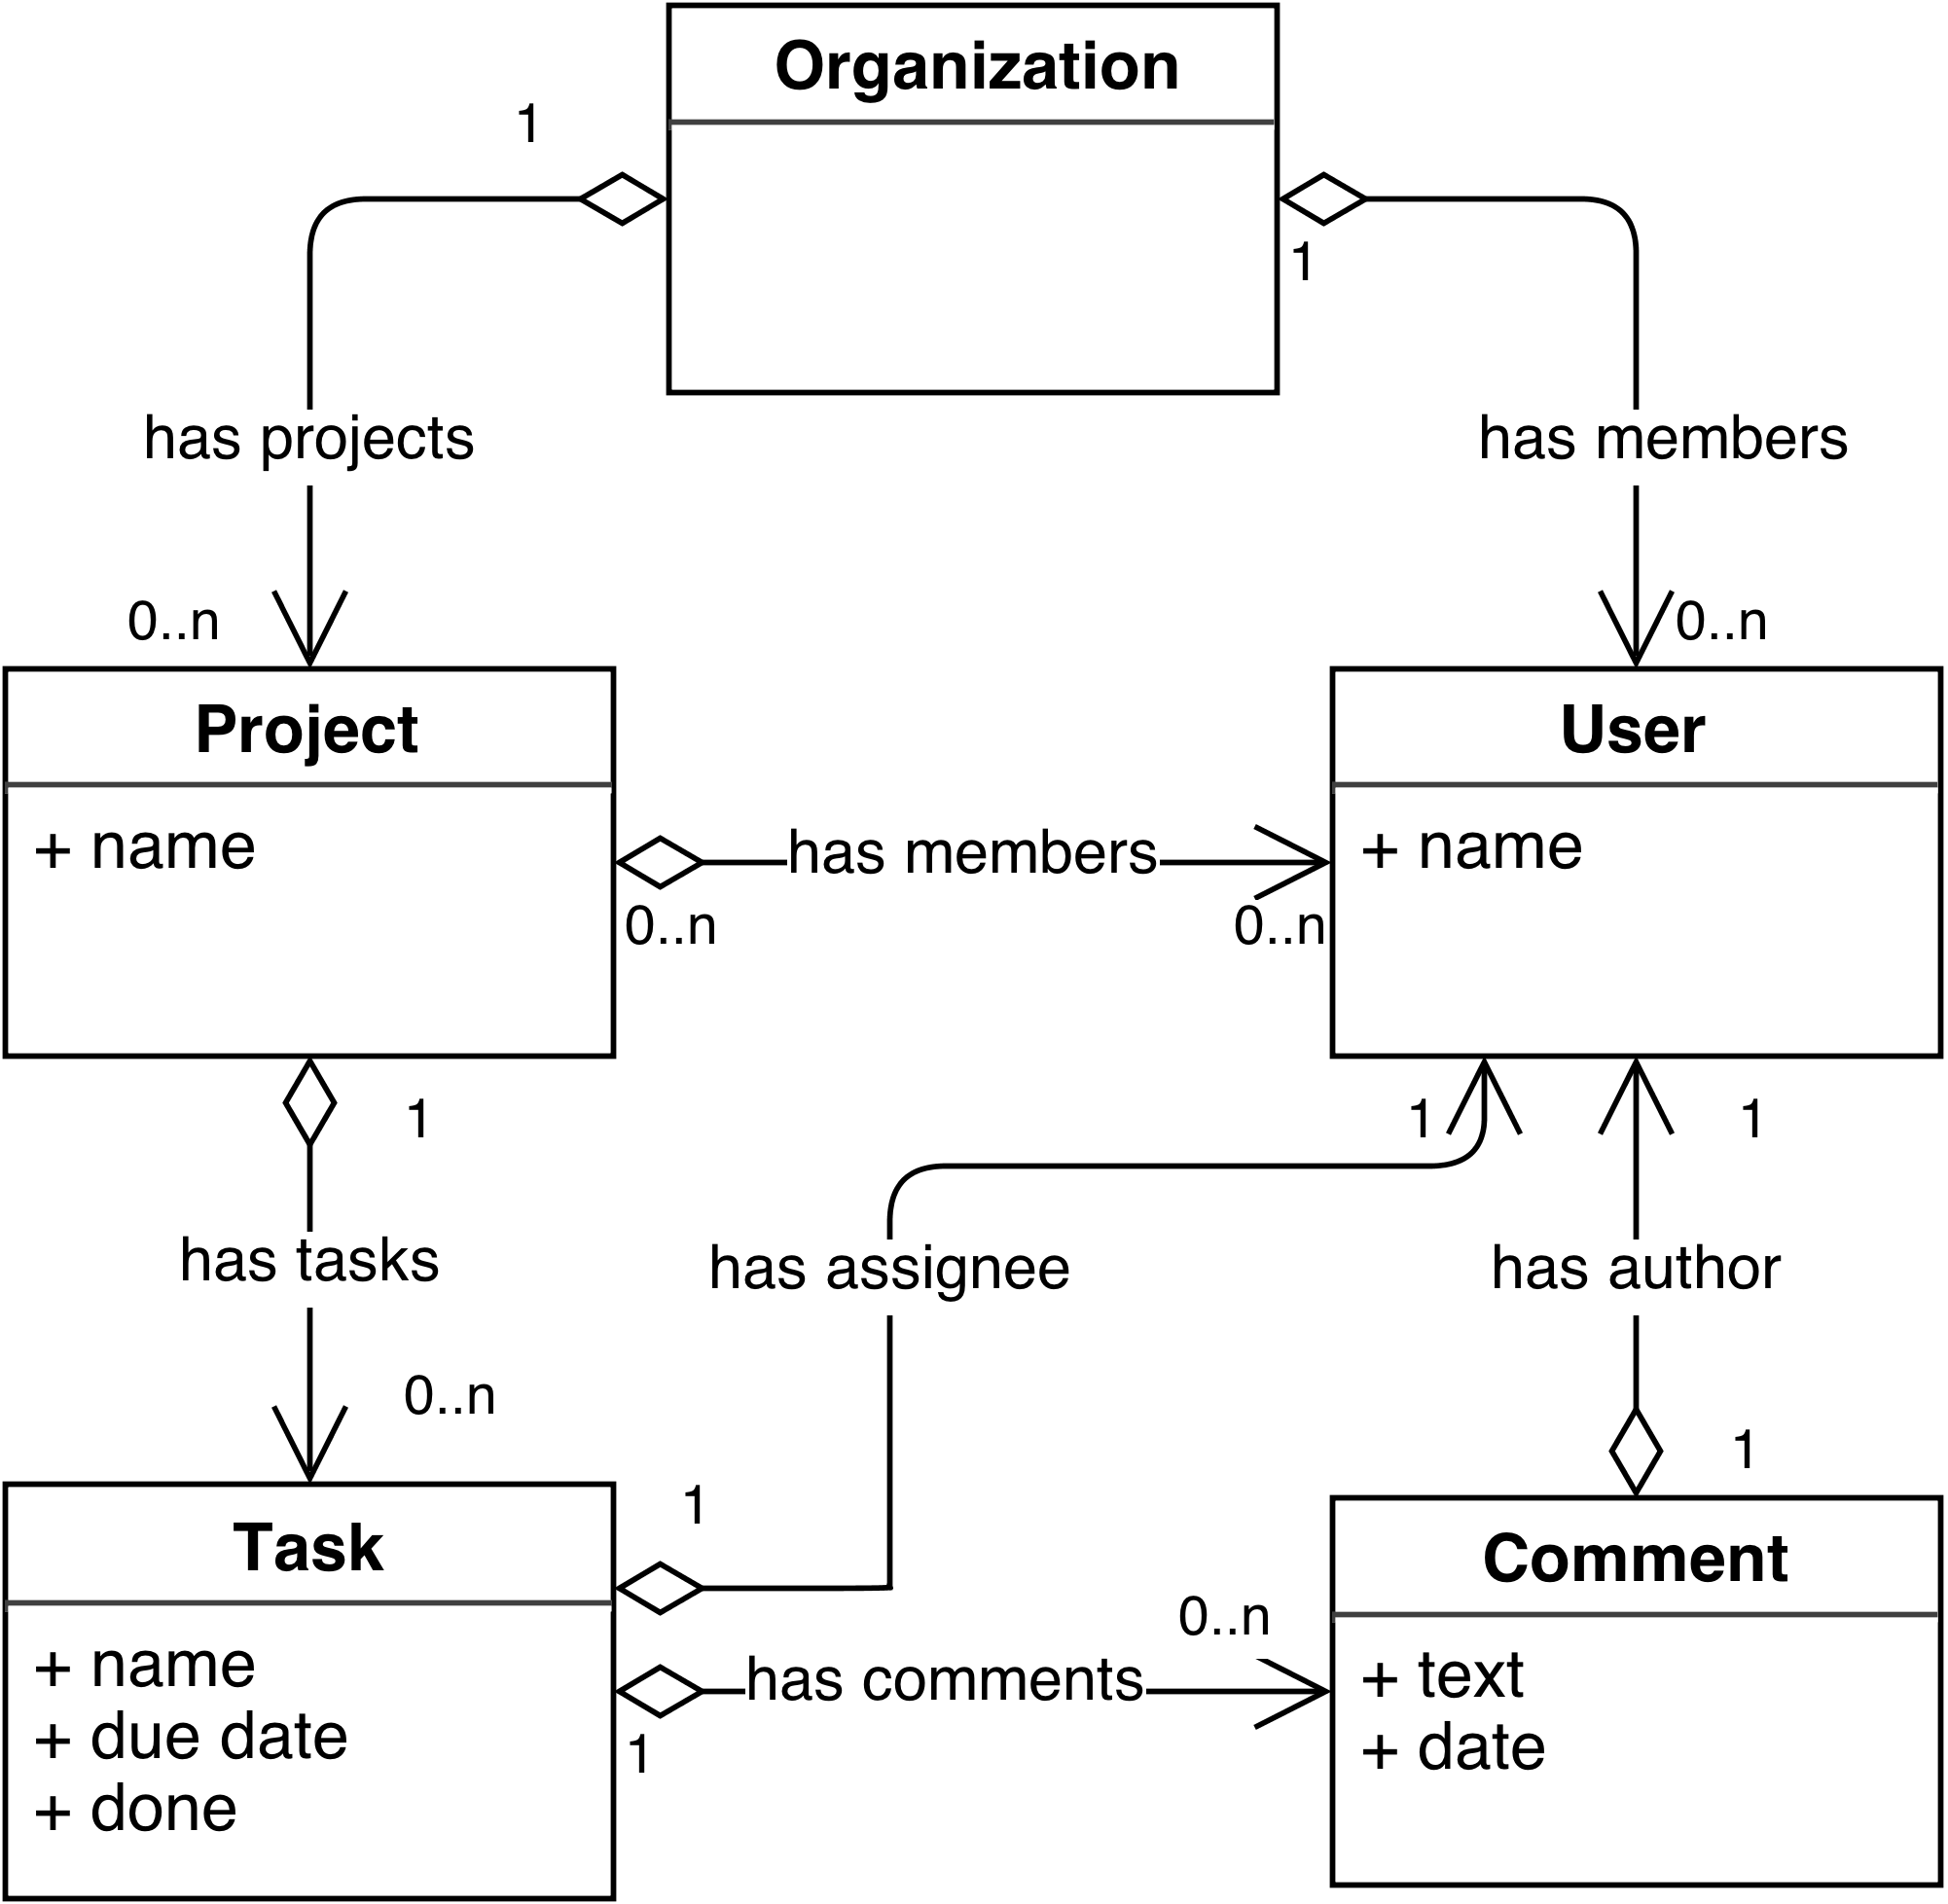
\includegraphics[width=0.8\textwidth]{img/tasks-schema}
\caption{A collaborative Task Manager's data schema}
\label{fig:tasks-data-schema}
\end{figure}
